
\usepackage{tikz}     % For graphics
\usepackage{amsmath, amssymb}  % For various math stuff
\usepackage{subfig}
\usepackage{centernot} % For the centernot macro
\usepackage{bbding}

\usetikzlibrary{arrows, automata, shapes.geometric, positioning, backgrounds}

\DeclareMathAlphabet{\mathitbf}{OML}{cmm}{b}{it}

%%%%%%%% COLOURS
\definecolor{darkgreen}{RGB}{0,128,0}


%%%%%%%%%%% HAXXXXORRR

\newenvironment{changemargin}[2]{%
\begin{list}{}{%
\setlength{\topsep}{0pt}%
\setlength{\leftmargin}{#1}%
\setlength{\rightmargin}{#2}%
\setlength{\listparindent}{\parindent}%
\setlength{\itemindent}{\parindent}%
\setlength{\parsep}{\parskip}%
}%
\item[]}{\end{list}}

%%%%%%%%%%%%%%% MATHEMATICAL NOTATIONS%%%%%%%%%
\newcommand{\defi}{\mathrel{{=_{\rm def}}}}
\newcommand{\abs}[1]{\lvert #1 \rvert}
\newcommand{\aut}[1]{\ensuremath{\mathcal{#1}}}
\newcommand{\set}[1]{\{ \, #1 \, \}}
\newcommand{\tuple}[1]{\langle \, #1 \, \rangle}
\newcommand{\suchthat}{\; . \;}
\newcommand{\project}{\mathrel{\upharpoonright}}
\newcommand{\where}{\mid}
\newcommand{\union}{\mathrel{\cup}}
\newcommand{\intersection}{\mathrel{\cap}}
\newcommand{\concat}{\mathrel{\cdot}}
\newcommand{\treq}{\ensuremath{\approx_{\mathrm{tr}} \;}}

\let\oldland\land
\let\oldlor\lor
\let\oldexists\exists
\let\oldforall\forall
\let\oldnexists\nexists

\renewcommand{\land}{\; \oldland \;}
\renewcommand{\lor}{\; \oldlor \;}
\renewcommand{\exists}{\, \oldexists \,}
\renewcommand{\forall}{\, \oldforall \,}
\renewcommand{\nexists}{\, \oldnexists \,}

\newcommand{\existsinfty}{\exists^{\infty}}
\newcommand{\fd}[1]{\ensuremath{\mathit{fd}(#1)}}
\newcommand{\pa}[1]{\ensuremath{\mathit{p}(#1)}}
\newcommand{\qu}[1]{\ensuremath{\mathit{q}(#1)}}
\newcommand{\blockedby}{\nmid}
%%%%%%%%%%%%%%% END MATHEMATICAL NOTATIONS%%%%%%

%%%%%%%%%%%%%%% RULES ETC %%%%%%%%%%%%%%%%%%
\newcounter{ruledefcounter}
\setcounter{ruledefcounter}{1}
\newenvironment{ruledef}[2]%
{\list{}{\leftmargin=0.1in\rightmargin=0in}\item[]\noindent\ignorespaces%
\textbf{Rule R\arabic{ruledefcounter}} %
(#1)%
\textbf{:} %
#2.\list{}{\leftmargin=0.1in\rightmargin=0in}\item[]}
{\endlist\stepcounter{ruledefcounter}\endlist\ignorespacesafterend}
%%%%%%%%%%%%%%% END RULES ETC %%%%%%%%%%%%%%%

%%%%%%%%%%%%%%% THEOREMS ETC %%%%%%%%%%%%%%%
%\theoremstyle{definition}
%\newtheorem{definition}{Definition}[section]
%\theoremstyle{plain}
%\newtheorem{lemma}[definition]{Lemma}
%\newtheorem{proposition}[definition]{Proposition}
%\newtheorem{theorem}[definition]{Theorem}
%\newtheorem{corollary}[definition]{Corollary}
%\theoremstyle{remark}
%\newtheorem{example}[definition]{Example}
%\newtheorem{remark}[definition]{Remark}
%
%\newcommand{\theoremlikeParameterised}[2]{\par\medskip\penalty-250\refstepcounter{definition}{\bfseries\scshape\noindent#1 #2.}\slshape}
%\newenvironment{theoremParam}[1]{\theoremlikeParameterised{\bf Theorem}{#1}}{\par\medskip}
%\newenvironment{lemmaParam}[1]{\theoremlikeParameterised{\bf Lemma}{#1}}{\par\medskip}
%\newenvironment{propositionParam}[1]{\theoremlikeParameterised{\bf Proposition}{#1}}{\par\medskip}
%%%%%%%%%%%%%%% END THEOREMS ETC %%%%%%%%%%%%

%%%%%%%%%%%%%%%% ARROWS %%%%%%%%%%%%%%%%
% auxiliaries
\newcommand{\linefill}{%
   \cleaders
   \hbox{$\smash{\mkern-2mu\mathord-\mkern-2mu}$}%
   \hfill
   \vphantom{\lower1pt\hbox{$\rightarrow$}}%
}

\newcommand{\Linefill}{%
   \cleaders
   \hbox{$\smash{\mkern-2mu\mathord=\mkern-2mu}$}%
   \hfill
   \vphantom{\hbox{$\Rightarrow$}}%
}

% left segment of extensible arrow, no ending
\newcommand{\xleftnoend}[1][]{\mathrel-_{\vphantom{#1}}\mkern-11mu}
\newcommand{\xLeftnoend}[1][]{\mathrel=_{\vphantom{#1}}\mkern-8mu}
% middle segment of extensible arrow
\newcommand{\xmid}[2][]{\stackrel{#2}{\linefill_{\vphantom{#1}}}}
\newcommand{\xMid}[2][]{\stackrel{#2}{\Linefill_{\vphantom{#1}}}}
% right segment of extensible arrow, arrow head
\newcommand{\xrightArrow}[1][]{\mkern-11mu\rightarrow_{#1}}
\newcommand{\xRightArrow}[1][]{\mkern-8mu\Rightarrow_{#1}}
% make arrow symbol
\newcommand{\xmake}[1]{\mathrel{\lower1pt\hbox{$#1$}}}

% single-arrow transition
\newcommand{\trans}[2][]{\xmake{\xleftnoend[#1]\xmid[#1]{#2}\xrightArrow[#1]}}
% negative single-arrow transition
\newcommand{\ntrans}[2][]{\centernot{\trans[#1]{#2}}}
% empty single-arrow transition
\newcommand{\etrans}{\rightarrow}

% double-arrow transition
\newcommand{\Trans}[2][]{\xmake{\xLeftnoend[#1]\xMid[#1]{#2}\xRightArrow[#1]}}
% negative double-arrow transition
\newcommand{\nTrans}[2][]{\centernot{\Trans[#1]{#2}}}
% empty double-arrow transition
\newcommand{\eTrans}{\Rightarrow}
%%%% END ARROWS %%%%%%%%%%%%%%%%%%%%%%%%%

%%%%%%%%%%%%%% TIKZ %%%%%%%%%%%%%%%%
\tikzstyle{background rectangle}= [rounded corners, fill=yellow!20, draw=black, rounded corners=1ex]
\tikzstyle{every picture}=[show background rectangle, ->,>=latex,auto,node distance=1.3cm,thick,initial text=,initial where=above,scale=0.9,transform shape]
\tikzstyle{every state}=[draw=yellow!20,line width=4pt,fill=black,minimum size=5pt]

\tikzstyle{loop right}=[in=-30,out=30,looseness=8]
\tikzstyle{loop left}=[in=150,out=210,looseness=8]
\tikzstyle{loop above}=[in=60,out=120,looseness=8]
\tikzstyle{loop below}=[in=240,out=300,looseness=8]

\tikzstyle{loop above right}=[in=5,out=65,looseness=8]
\tikzstyle{loop above left}=[in=105,out=165,looseness=8]
\tikzstyle{loop slightly above left}=[in=125,out=185,looseness=8]
\tikzstyle{loop slightly above right}=[in=5,out=65,looseness=8]
\tikzstyle{loop below left}=[in=195,out=255,looseness=8]
\tikzstyle{loop below right}=[in=285,out=-15,looseness=8]
\tikzstyle{loop slightly below left}=[in=155,out=215,looseness=8]
\tikzstyle{loop slightly below right}=[in=305,out=5,looseness=8]

\tikzstyle{nodeSmall} = [state, node distance=1.5cm, draw=yellow!20, fill=black]
\tikzstyle{finalNode} = [node distance=1.5cm]
\newcommand{\back}{\color{yellow!20}mm}
\tikzstyle{onEdge}=[fill=yellow!20, pos=0.5]
%%%%%%%%%%%%%% END TIKZ %%%%%%%%%%%%%

%%%%%%%%%%%%%% USEFUL ALIASES %%%%%%%%%
\newcommand{\ioco}{\texttt{ioco}}

\newcommand{\impl}{\aut{A}_i}
\newcommand{\spec}{\aut{A}_s}
\newcommand{\ioconf}{\sqsubseteq_{\ioco}}

\newcommand{\AparB}{\ensuremath{\aut{A} \parallel \aut{B}}}
\newcommand{\AparBie}{\ensuremath{\aut{A} \parallel_{\rm I} \aut{B}}}

\newcommand{\Lin}{L^{\text{\rm I}}}
\newcommand{\Lout}{L^{\text{\rm O}}}
\newcommand{\Ltau}{L^{\tau}}
\newcommand{\Ldelta}{L^{\delta}}
\newcommand{\Ltaudelta}{L^{\delta}_{\tau}}
\newcommand{\LA}{L_{\aut{A}}}
\newcommand{\LB}{L_{\aut{B}}}
\newcommand{\LC}{L_{\aut{C}}}
\newcommand{\LD}{L_{\aut{D}}}
\newcommand{\LinA}{\Lin_{\aut{A}}}
\newcommand{\LinB}{\Lin_{\aut{B}}}
\newcommand{\LinC}{\Lin_{\aut{C}}}
\newcommand{\LinD}{\Lin_{\aut{D}}}
\newcommand{\LoutA}{\Lout_{\aut{A}}}
\newcommand{\LoutB}{\Lout_{\aut{B}}}
\newcommand{\LoutC}{\Lout_{\aut{C}}}
\newcommand{\LoutD}{\Lout_{\aut{D}}}
\newcommand{\LoutHide}{\Lout_{H}}
\newcommand{\LtauA}{\Ltau_{\aut{A}}}
\newcommand{\LtauB}{\Ltau_{\aut{B}}}
\newcommand{\LtauC}{\Ltau_{\aut{C}}}
\newcommand{\LtauD}{\Ltau_{\aut{D}}}
\newcommand{\LtauHide}{\Ltau_{H}}
\newcommand{\LdeltaA}{\Ldelta_{\aut{A}}}
\newcommand{\LdeltaB}{\Ldelta_{\aut{B}}}
\newcommand{\LdeltaC}{\Ldelta_{\aut{C}}}
\newcommand{\LdeltaD}{\Ldelta_{\aut{D}}}
\newcommand{\LAparB}{L_{\AparB}}
\newcommand{\LinAparB}{\Lin_{\AparB}}
\newcommand{\LoutAparB}{\Lout_{\AparB}}
\newcommand{\LtauAparB}{\Ltau_{\AparB}}
\newcommand{\LdeltaAparB}{\Ldelta_{\AparB}}

\newcommand{\sdelta}{s_{\delta}}
\newcommand{\fdelta}{f_{\delta}}

\newcommand{\SA}{S_{\aut{A}}}
\newcommand{\SB}{S_{\aut{B}}}
\newcommand{\SC}{S_{\aut{C}}}
\newcommand{\SD}{S_{\aut{D}}}
\newcommand{\SAparB}{S_{\AparB}}
\newcommand{\Sdelta}{S_{\delta}}
\newcommand{\Shide}{S_{H}}

\newcommand{\Sstart}{S^0}
\newcommand{\SstartA}{\Sstart_{\aut{A}}}
\newcommand{\SstartB}{\Sstart_{\aut{B}}}
\newcommand{\SstartC}{\Sstart_{\aut{C}}}
\newcommand{\SstartD}{\Sstart_{\aut{D}}}
\newcommand{\SstartAparB}{\Sstart_{\AparB}}

\newcommand{\PA}{P_{\aut{A}}}
\newcommand{\PB}{P_{\aut{B}}}
\newcommand{\PC}{P_{\aut{C}}}
\newcommand{\PD}{P_{\aut{D}}}
\newcommand{\PAparB}{P_{\AparB}}

\newcommand{\transA}[2][]{\trans[#1]{#2}_{\aut{A}}}
\newcommand{\transB}[2][]{\trans[#1]{#2}_{\aut{B}}}
\newcommand{\transC}[2][]{\trans[#1]{#2}_{\aut{C}}}
\newcommand{\transD}[2][]{\trans[#1]{#2}_{\aut{D}}}
\newcommand{\transAparB}[2][]{\trans[#1]{#2}_{\AparB}}
\newcommand{\transAparBie}[2][]{\trans[#1]{#2}_{\AparBie}}
\newcommand{\transDelta}[2][]{\trans[#1]{#2}_{\delta}}
\newcommand{\transDet}[2][]{\trans[#1]{#2}_{\mathrm{D}}}
\newcommand{\transHide}[2][]{\trans[#1]{#2}_{H}}
\newcommand{\transDeltaHide}[2][]{\trans[#1]{#2}_{\delta(\mathrm{H})}}
\newcommand{\transHideDelta}[2][]{\trans[#1]{#2}_{\mathrm{H}(\delta)}}

\newcommand{\TransA}[2][]{\Trans[#1]{#2}_{\aut{A}}}
\newcommand{\TransB}[2][]{\Trans[#1]{#2}_{\aut{B}}}
\newcommand{\TransC}[2][]{\Trans[#1]{#2}_{\aut{C}}}
\newcommand{\TransD}[2][]{\Trans[#1]{#2}_{\aut{D}}}
\newcommand{\TransAparB}[2][]{\Trans[#1]{#2}_{\AparB}}
\newcommand{\TransAparBie}[2][]{\Trans[#1]{#2}_{\AparBie}}
\newcommand{\TransDelta}[2][]{\Trans[#1]{#2}_{\delta}}
\newcommand{\TransDet}[2][]{\Trans[#1]{#2}_{\mathrm{D}}}
\newcommand{\TransHide}[2][]{\Trans[#1]{#2}_{H}}
\newcommand{\TransHideDelta}[2][]{\Trans[#1]{#2}_{\mathrm{H}(\delta)}}

\newcommand{\ntransA}[2][]{\ntrans[#1]{#2}_{\aut{A}}}
\newcommand{\ntransB}[2][]{\ntrans[#1]{#2}_{\aut{B}}}
\newcommand{\ntransC}[2][]{\ntrans[#1]{#2}_{\aut{C}}}
\newcommand{\ntransD}[2][]{\ntrans[#1]{#2}_{\aut{D}}}
\newcommand{\ntransAparB}[2][]{\ntrans[#1]{#2}_{\AparB}}
\newcommand{\ntransAparBie}[2][]{\ntrans[#1]{#2}_{\AparBie}}
\newcommand{\ntransDelta}[2][]{\ntrans[#1]{#2}_{\delta}}
\newcommand{\ntransHide}[2][]{\ntrans[#1]{#2}_{H}}
\newcommand{\ntransDet}[2][]{\ntrans[#1]{#2}_{\mathrm{D}}}

\newcommand{\nTransA}[2][]{\nTrans[#1]{#2}_{\aut{A}}}
\newcommand{\nTransB}[2][]{\nTrans[#1]{#2}_{\aut{B}}}
\newcommand{\nTransC}[2][]{\nTrans[#1]{#2}_{\aut{C}}}
\newcommand{\nTransD}[2][]{\nTrans[#1]{#2}_{\aut{D}}}
\newcommand{\nTransAparB}[2][]{\nTrans[#1]{#2}_{\AparB}}
\newcommand{\nTransAparBie}[2][]{\nTrans[#1]{#2}_{\AparBie}}
\newcommand{\nTransDelta}[2][]{\nTrans[#1]{#2}_{\delta}}
\newcommand{\nTransDet}[2][]{\nTrans[#1]{#2}_{\mathrm{D}}}
\newcommand{\nTransHide}[2][]{\nTrans[#1]{#2}_{H}}

\newcommand{\etransA}{\etrans_{\aut{A}}}
\newcommand{\etransB}{\etrans_{\aut{B}}}
\newcommand{\etransC}{\etrans_{\aut{C}}}
\newcommand{\etransD}{\etrans_{\aut{D}}}
\newcommand{\etransAparB}{\etrans_{\AparB}}
\newcommand{\etransAparBie}{\etrans_{\AparBie}}
\newcommand{\etransDelta}{\etrans_{\delta}}
\newcommand{\etransDet}{\etrans_{\mathrm{D}}}
\newcommand{\etransHide}{\etrans_{H}}
\newcommand{\etransDeltaHide}{\etrans_{\delta(\mathrm{H})}}
\newcommand{\etransHideDelta}{\etrans_{\mathrm{H}(\delta)}}

\newcommand{\deltaf}[1]{\ensuremath{\delta(#1)}}
\newcommand{\deter}[1]{\ensuremath{\mathit{det}(#1)}}
\newcommand{\hide}[2]{\ensuremath{#1 \setminus #2}}
\newcommand{\init}[1]{\ensuremath{\mathit{init}(#1)}}
\newcommand{\trace}[1]{\ensuremath{\mathit{trace}(#1)}}
\newcommand{\states}[1]{\ensuremath{\mathit{states}(#1)}}
\newcommand{\paths}[1]{\ensuremath{\mathit{paths}(#1)}}
\newcommand{\dpaths}[1]{\ensuremath{\mathit{dpaths}(#1)}}
\newcommand{\fpaths}[1]{\ensuremath{\mathit{fpaths}(#1)}}
\newcommand{\fdpaths}[1]{\ensuremath{\mathit{fdpaths}(#1)}}

\newcommand{\rs}[1]{\ensuremath{\mathit{rs}_{#1}}}
\newcommand{\qos}[1]{\ensuremath{\mathit{qos}_{#1}}}

\newcommand{\fdclosures}[1]{\ensuremath{\mathit{fdclosures}(#1)}}
\newcommand{\newfdclosures}[1]{\ensuremath{\mathit{new\text{-}fdclosures}(#1)}}

\newcommand{\reach}[1]{\ensuremath{\mathit{reach}(#1)}}
\newcommand{\reachA}[1]{\ensuremath{\mathit{reach}_{\aut{A}}(#1)}}
\newcommand{\reachB}[1]{\ensuremath{\mathit{reach}_{\aut{B}}(#1)}}
\newcommand{\reachAparB}[1]{\ensuremath{\mathit{reach}_{\AparB}(#1)}}
\newcommand{\reachHide}[1]{\ensuremath{\mathit{reach}_{H}(#1)}}

\newcommand{\traces}[1]{\ensuremath{\mathit{traces}(#1)}}
\newcommand{\tracesA}[1]{\ensuremath{\mathit{traces}_{\aut{A}}(#1)}}
\newcommand{\tracesB}[1]{\ensuremath{\mathit{traces}_{\aut{B}}(#1)}}
\newcommand{\tracesAparB}[1]{\ensuremath{\mathit{traces}_{\AparB}(#1)}}
\newcommand{\tracesDelta}[1]{\ensuremath{\mathit{traces}_{\delta}(#1)}}
\newcommand{\tracesDet}[1]{\ensuremath{\mathit{traces}_{\mathrm{D}}(#1)}}
\newcommand{\tracesHide}[1]{\ensuremath{\mathit{traces}_{H}(#1)}}
\newcommand{\tracesDeltaHide}[1]{\ensuremath{\mathit{traces}_{\delta(\mathrm{H})}(#1)}}
\newcommand{\tracesHideDelta}[1]{\ensuremath{\mathit{traces}_{\mathrm{H}(\delta)}(#1)}}
%%%%%%%%%%% END USEFUL ALIASES  %%%%%%%%%

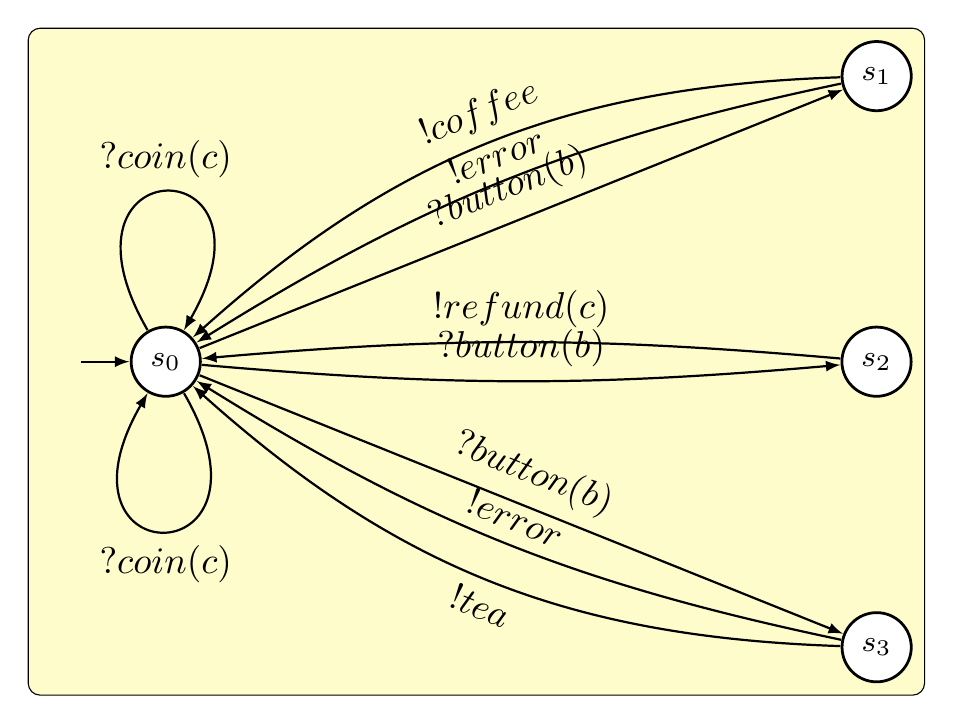
\begin{tikzpicture}[scale=1.5]
	\tikzstyle{every state}=[draw=black,line width=1pt,fill=white,minimum size=5pt]

	\node[state, initial left] (s0) {\footnotesize $s_0$};
  \node[state] (s2) [right=6cm of s0] {\footnotesize $s_2$};
	\node[state] (s1) [above=2cm of s2] {\footnotesize $s_1$};
  \node[state] (s3) [below=2cm of s2] {\footnotesize $s_3$};
	
	\path (s0) edge[min distance=20mm,loop above] node [above] {$?coin(c)$ } (s0) ;
  \path (s0) edge[min distance=20mm,loop below] node [below] {$?coin(c)$ } (s0) ;
	\path (s0) edge node [sloped,midway,above] {$?button(b)$} (s1) ;
  \path (s0) edge[bend right=5] node [sloped,midway,above] {$?button(b)$} (s2) ;
  \path (s0) edge node [sloped,midway,above] {$?button(b)$} (s3) ;
	\path (s1) edge[bend right=20] node [sloped,midway,above] {$!coffee$} (s0) ;
  \path (s1) edge[bend right=10] node [sloped,midway,above] {$!error$} (s0) ;
  \path (s2) edge[bend right=5] node [sloped,midway,above] {$!refund(c)$} (s0) ;
  \path (s3) edge[bend left=20] node [sloped,midway,below] {$!tea$} (s0) ;
  \path (s3) edge[bend left=10] node [sloped,midway,above] {$!error$} (s0) ;
\end{tikzpicture}
